% ==============================================================================================
\chapter{Dynamic point load on elastic halfspace}\label{ch:pekeris}
% ==============================================================================================

% ----------------------------------------------------------------------------------------------
\section{Introduction}
% ----------------------------------------------------------------------------------------------
This benchmark compares the STEM numerical solution against the analytical solution
for a dynamic point load applied to the surface of an elastic half-space (known as the Lamb problem).

The analytical solution was derived by Pekeris and is detailed in~\cite{Verruijt_2010}.
The analytical solution provides closed-form expressions for the vertical displacement along the surface of the
half-space, enabling a direct time-history comparison against the numerical model.


% ----------------------------------------------------------------------------------------------
\section{Model Description}
% ----------------------------------------------------------------------------------------------

% ..............................................................................................
\subsection{Geometry, mesh and loading}
% ..............................................................................................
The point load was modelled in a three-dimensional domain representing an elastic half-space.
An overview of the geometry for the numerical analysis is shown in Figure~\ref{fig:3D_scheme}.
The soil has a width and length of \qty{10}{\meter} and depth of \qty{5}{\meter} and is subjected to a
compressive pulse load, $F(t)$, which is suddenly applied at the top edge:

\begin{equation}
    F(t) =
     \begin{cases}
    0, & \text{if } t<0\\
    \qty{-1000}{\kilo\newton}, & \text{if } t>0\\
    \end{cases}
\end{equation}


\begin{figure}
    \centering
    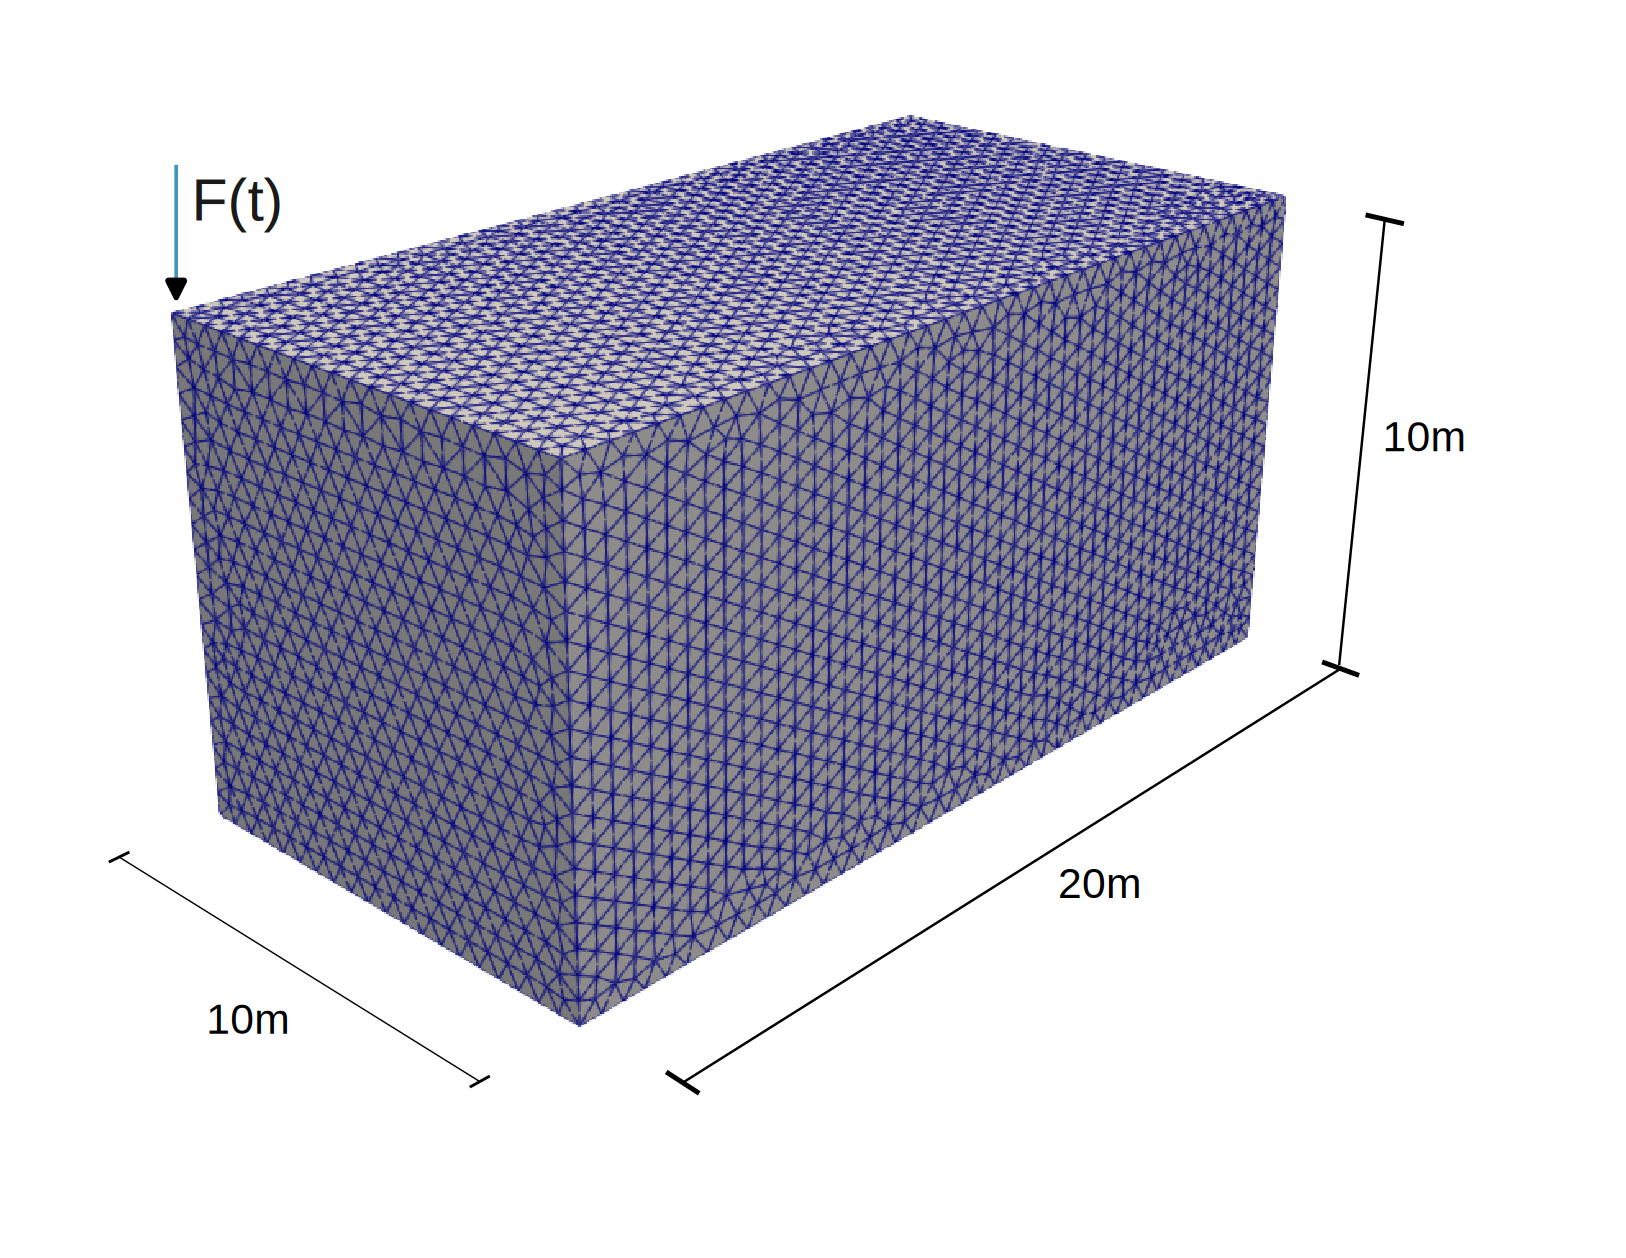
\includegraphics[width=0.75\textwidth]{lamb/mesh.pdf}
    \caption{Geometry, mesh and loading conditions for the three-dimensional wave propagation problem.}
    \label{fig:3D_scheme}
\end{figure}

The soil is discretised in second-order tetrahedral elements with size \qty{0.25}{\meter}.
Absorbing boundary conditions are applied at the free ends of the lateral boundaries, while fixed boundary
conditions are imposed on the perpendicular plane along the axis of symmetry.
At the bottom the soil is assumed to be fixed, simulating the existence of the top of bedrock that has a
significantly larger stiffness than the soil above.

% ..............................................................................................
\subsection{Materials and numerical parameters}
% ..............................................................................................
The soil is modelled as a one-phase continuum with a linear elastic constitutive law, with the
following parameters:

\begin{itemize}[noitemsep,topsep=0pt,parsep=0pt,partopsep=0pt]
    \item Young's modulus: \qty{30}{\mega\pascal},
    \item Poisson ratio: \qty{0.3},
    \item Density: \qty{2000}{\kilogram\per\meter\cubed}.
\end{itemize}

Material damping is included via Rayleigh damping, with parameters that provide a damping ratio of
\qty{0.01}{\percent} at \qty{1}{\hertz} and \qty{80}{\hertz}.

The dynamic analysis is performed over a \qty{0.08}{\second} time window, with a time step of \qty{0.001}{\second}.
The system of equations is solved using the Newmark time integration~\cite{Newmark_1959} scheme with
parameters $\beta = 0.25$ and $\gamma = 0.5$.

% ----------------------------------------------------------------------------------------------
\section{Results}
% ----------------------------------------------------------------------------------------------
Figure~\ref{fig:pekeris_results} presents the time histories of the vertical displacement for three
nodes, located at 1, 2 and~\qty{3}{\meter} from the load, located along the surface.
The figure compares the STEM results against the analytical solution.
If follows that there is an agreement between both solutions, demonstrating the accuracy of the STEM
for this type of dynamic loading condition. This is a notable difficult problem to solve numerically,
due to the steep gradients in stress and displacement that occur close to the point of application of the
load.

\begin{figure}[h]
    \centering
    \includegraphics[width=0.8\textwidth]{lamb/time_history.pdf}
    \caption{Comparison of the vertical displacement time histories at surface nodes located at:
     (a) \qty{1}{\meter}, (b) \qty{2}{\meter} and (c) \qty{3}{\meter} from the load.}
    \label{fig:pekeris_results}
\end{figure}
